%File: formatting-instruction.tex
\documentclass[letterpaper]{article}
\usepackage{aaai}
\usepackage{times}
%\usepackage{hyperref}
\usepackage{graphicx}
\usepackage{subfigure}
\frenchspacing
\setlength{\pdfpagewidth}{8.5in}
\setlength{\pdfpageheight}{11in}
\usepackage{amsmath}
%\pdfinfo{
%/Title ( Error Classification in OCR Historic Newspaper Archive using SVM\textsuperscript{multiclass})
%/Author (Megha Gupta, Dr. Haimonti Dutta)}
\setcounter{secnumdepth}{1}  
 \begin{document}
% The file aaai.sty is the style file for AAAI Press 
% proceedings, working notes, and technical reports.
%
%\title{Crowdsourced OCR Error Correction Classification using Multi-Class Support Vector Machines}
%\title{Classification of Text Corrected by the Crowd using Support Vector Machines}
\title{ \textbf{C}lassification of \textbf{C}rowdsourced \textbf{T}ext \textbf{C}orrection}
%\author{Megha Gupta\\Department of Computer Science,\\ IIIT-Delhi, India \\ meghag@iiitd.ac.in 
%\And Dr. Haimonti Dutta\\
%Center for Computational Learning Systems,\\ Columbia University, New York\\ haimonti@iiitd.ac.in}

\author{Haimonti Dutta\thanks{The author is also a visiting assistant professor at IIIT-Delhi.}\\
Center for Computational Learning Systems, \\
Columbia University, \\
New York, NY 10115\\
haimonti@ccls.columbia.edu\\
\And
Megha Gupta \\
Dept. of Computer Science\\ 
IIIT-Delhi, India. \\
meghag@iiitd.ac.in
\And 
Brian Geiger \\
Center for Bibliographical Studies and Research \\
University of California, Riverside \\
brian.geiger@ucr.edu
}

\maketitle
\begin{abstract}
\begin{quote}
\noindent Optical Character Recognition (OCR) is a commonly used technique for digitizing printed material enabling them to be displayed online, searched and used in text mining applications. 
The text generated from OCR devices is often garbled due to variations in quality of the input paper, size and style of the font and column layout. This adversely affects retrieval effectiveness and hence techniques for cleaning the garbled text need to be improvised. Often such techniques involve laborious and time consuming manual processing of data. This paper presents a prototype system for \textbf{C}lassification of \textbf{C}rowdsourced \textbf{T}ext \textbf{C}orrection (CCTC) which takes as input log files containing garbled and manually corrected OCR text, parses and tokenizes them and builds models for categorizing the corrections using state-of-the-art machine learning algorithms. Retrieval effectiveness on the California Digital Newspaper Collection is measured using Spearman's rank correlation metric. This prototype system is expected to be deployed on historical newspaper archives that make extensive use of user text corrections.
\end{quote}
\end{abstract}

\section{Introduction}
\label{sec:intro}

Crowdsourcing is used extensively in cultural heritage and digital history related projects in recent years to 
%<<<<<<< HEAD
%digitize, create and process content and provide editorial or processing interventions. For example, the Australian Newspapers Digitization Program \cite{ADNP} enables communities to explore their rich newspaper heritage by enabling free online public access to over 830,000 newspaper pages containing 8.4 million articles. The public enhanced the data by correcting over 7 million lines of text and adding 200,000 tags and 4600 comments \cite{holley_09}. Picture Australia \cite{pictAus} harvests digital images from other heritage institutions and encourages the public to upload their own images and tag them. FamilySearch \cite{famSearch} made available handwritten digital images of births, deaths and marriage records for transcription by the public. The New York Public Library has 1,277,616 dishes transcribed to date from 17,079 menus. Galaxy Zoo \cite{galZoo} is an online collaborative astronomy project in which users are invited to classify millions of galaxies from digital photos. 
%
%In all of the above crowdsourcing projects, large volumes of data are generated by users. These include tags, folksonomies, flagged content, information on history, relationship and preference data, structured labels describing objects and creative responses \cite{Ridge_11}. In most citizen science projects, however, little statistical analysis is done on the user generated content. Thus assessment of data quality obtained by leveraging the ``wisdom of the crowd" remains an open problem. 
%=======
digitize, create and process content and provide editorial or processing interventions. For example, the Australian Newspapers Digitization Program \cite{ADNP} allows communities to explore their rich newspaper heritage by enabling free online public access to over 830,000 newspaper pages containing 8.4 million articles. The public enhanced the data by correcting over 7 million lines of text and adding 200,000 tags and 4600 comments \cite{holley_09}. 
%Picture Australia \cite{pictAus} harvests digital images from other heritage institutions and encourages the public to upload their own images and tag them. 
FamilySearch \cite{famSearch} made available handwritten digital images of births, deaths and marriage records for transcription by the public. The New York Public Library has 1,277,616 dishes transcribed to date from 17,079 menus. 
%Galaxy Zoo \cite{galZoo} is an online collaborative astronomy project in which users are invited to classify millions of galaxies from digital photos. 

In all of the above crowdsourcing projects, large volumes of data are generated by users. These include tags, folksonomies, flagged content, information on history, relationship and preference data, structured labels describing objects and creative responses \cite{Ridge_11}. However, little statistical analysis is done of the user generated content in most cases. Assessment of data quality obtained by leveraging the ``wisdom of the crowd" remains an open problem. 

%Before this question can be answered, statistical analysis of the data generated is imperative.

In this paper, we focus on understanding the nature of text corrections done by users of an old historic newspaper archive. The newspapers are made available for searching on the Internet after the following processes take place: (1) the microfilm copy or paper original is scanned; %(2) master and Web image files are generated; 
(2) metadata is assigned for each page to improve the search capability of the newspaper; (3) OCR software is run over high resolution images to create searchable full text.
% and (5) OCR text, images, and metadata are imported into a digital library software program. 
The OCR scanning process is far from perfect and the documents generated from it contains a large amount of garbled text. A user is presented with a high resolution image of a newspaper page along with erroneous or distorted text from the OCR and is expected to rectify the garbled words as appropriate. A prototype for a system that can be used for \textbf{C}lassification of \textbf{C}rowdsourced \textbf{T}ext \textbf{C}orrection (CCTC) is presented which can answer simple questions such as ``What are the different kinds corrections proposed by users?" and provide statistics generated from the correction process. The output from the system can be used to enhance search and retrieval.

The study used log files generated from text correction software in use at the California Digital Newspaper Collection (CDNC)\footnote{http://cdnc.ucr.edu/cgi-bin/cdnc}, which contains over 400,000 pages of newspapers published in California between 1846-1922. 
%To date, the archive has approximately 1680 registered users who have corrected close to 2 million lines of text. 
%The corrections are primarily categorized as changes in spellings, punctuation rectification, addition of content or capitalization. A semi-automatic engine for classifying corrections based on support vector machines is designed.  
To the best of our knowledge, this is the first attempt to statistically analyze and model OCR error corrections provided by the crowd. We posit that such a classification system will be beneficial when attempting to compensate the annotators; it can also be used for task allocation if some users are more comfortable with certain type of corrections than others.

%In a bid to serve its patrons better, the CDNC crowdsourced the cleaning of OCR text. To date..
\begin{figure*}[t]
\centering
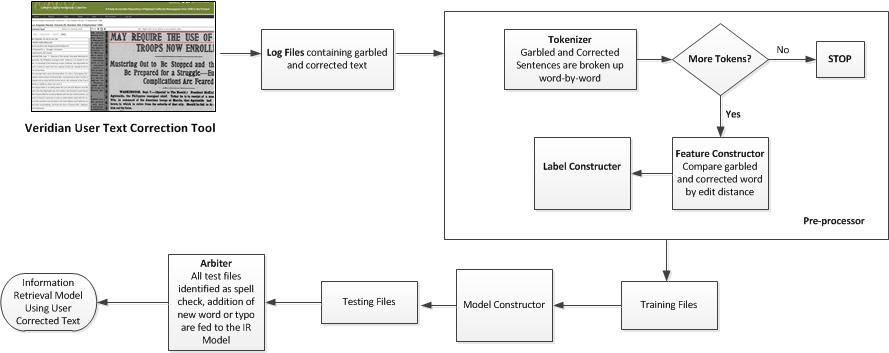
\includegraphics[width=0.8\textheight]{./image/archOCR.jpg}
\caption{The Architecture of the Proposed System}
\label{fig:arch}
\end{figure*}



\noindent \textbf{Organization}: Section~\ref{arch} describes the architecture of the proposed system; Section~\ref{sec:evaluation} presents empirical and scalability results on real-world data collected at CDNC; Section~\ref{ir} presents information retrieval techniques; Section~\ref{sec:related} discusses related work. Finally, Section~\ref{sec:conc} concludes the paper.



%The \textit{California Digital Newspaper Collection}\footnote{http://cdnc.ucr.edu/cgi-bin/cdnc} is an initiative of the Center for Bibliographical Studies and Research (CBSR) which is supported in part by the U.S. Institute of Museum and Library Services. It is also supported by the National Endowment for the Humanities (NEH) to digitise California newspapers for the National Digital Newspaper Program (NDNP). It contains over 400,000 pages of significant historical California newspapers published from 1846-1922.\\
%OCR devices are widely used in electronic conversion of scanned images which are handwritten or printed text into a machine encoded text. It finds most successful applications in the field of machine Learning, Artificial Intelligence and Pattern recognition. It deals with the problem of recognising optically generated characters be it offline or online. The performance directly depends on the quality of input document. The more constrained the input is the better will be the performance of the system. But when it comes to unconstrained handwriting, the performance is far from satisfactory. The main application areas for \cite{OCR} like Automatic number plate readers, form readers, signature verification.\\
%This project deals with printed text in the form of Historical Newspaper Articles in the holdings of \cite{cdnc}. One such newspaper, The Amador Ledger published in the early 1900s by the Amador Publishing Company appealed to the community's interests by covering issues unique to gold mining. Patrons of the \cite{cdnc} continue to be interested in studying about the status of the local mining industry and consequently read the Amador Ledger on a regular basis even to this day and correct \cite{OCR} errors as they come across them.\\
%In this paper, we perform error classification using Joachims multi-class Support Vector Machine algorithm called \textit{SVM\textsuperscript{multiclass}}\footnote{http://www.cs.cornell.edu/people/tj/svm\_light/svm\_multiclass.html}. We chose this algorithm as its the state of the art algorithm till now. But the experiments give altogether a different view on this algorithm. This algorithm do not converge quickly on certain parameters which are shown in table ~\ref{table: runtime}


\begin{figure*}[t]
\centering
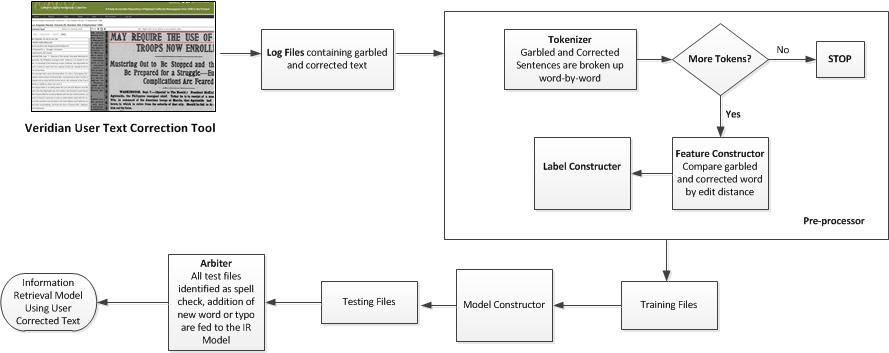
\includegraphics[width=0.8\textheight]{./image/archOCR.jpg}
\caption{The Architecture of the Proposed System}
\label{fig:arch}
\end{figure*}

\section{Architecture of the Proposed System}
\label{arch}


The \textbf{C}lassification of \textbf{C}rowdsourced \textbf{T}ext \textbf{C}orrection (CCTC) system has the following components:

\begin{enumerate}

\item The \textbf{Veridian User Text Correction}\footnote{http://veridiansoftware.com/crowdsourcing/} tool which takes as input a scanned page of the newspaper and enables users to correct OCR errors as they come across them.
Figure~\ref{fig:T1} shows an example of a scanned page from ``The Amador Ledger" published on January 26, 1900. The article to be corrected by a user is highlighted. The raw OCR text from the article and the tool used by patrons to correct text is shown in figure ~\ref{fig:T2}.


\item \textbf{Log Files: }All corrections performed by the annotators are recorded in log files. To date approximately 1,705,149 lines have been edited by 848 annotators which resulted in 235 log files. A sample of 191 files has been used for this work. Each log file is generated at the issue-level and contains XML data about the pages in the issue. Table~\ref{table:logfile} describes the structure of the log file. The following information is provided about the corrections made by the patrons:
%\begin{enumerate}
(a) \textit{Page Id: } The id of the page in which editing was done.
(b) \textit{Block Id: } The id of the paragraph containing the line corrected by the user.
(c) \textit{Line Id: }The id of the line edited by the user.
(d) \textit{Old Text Value} is the garbled text generated by the OCR device and replaced by the user.
(e) \textit{New Text Value} is the corrected text with which the old text was replaced.
%\end{enumerate}

\begin{table}[h]
\begin{center}
\begin{tabular}{l}
\textless TextCorrectedLine lineID="P2\_TL00800"\textgreater \\
\textless OldTextValue\textgreater \textbf{Spll, Stales}\textless /OldTextValue\textgreater \\
\textless NewTextValue\textgreater \textbf{Union Stables}\textless /NewTextValue\textgreater \\
\textless /TextCorrectedLine\textgreater \\
\textless TextCorrectedLine lineID="P2\_TL00801"\textgreater \\
\textless OldTextValue\textgreater \textbf{**?�** Under Webb Hall *}\textless/OldTextValue\textgreater \\
\textless NewTextValue\textgreater \textbf{Under Webb Hall} \textless/NewTextValue\textgreater \\
\textless /TextCorrectedLine\textgreater \\
\end{tabular}
\end{center}
\caption{A segment of the log file}
\label{table:logfile}
\end{table}

\begin{figure*}[th]
\begin{center}
%\mbox{
\subfigure[Scanned newspaper highlighting an article to be corrected by a user.]
{
%%\includegraphics[width=0.6\columnwidth]{odds_20070813_160000rb_M.pdf}
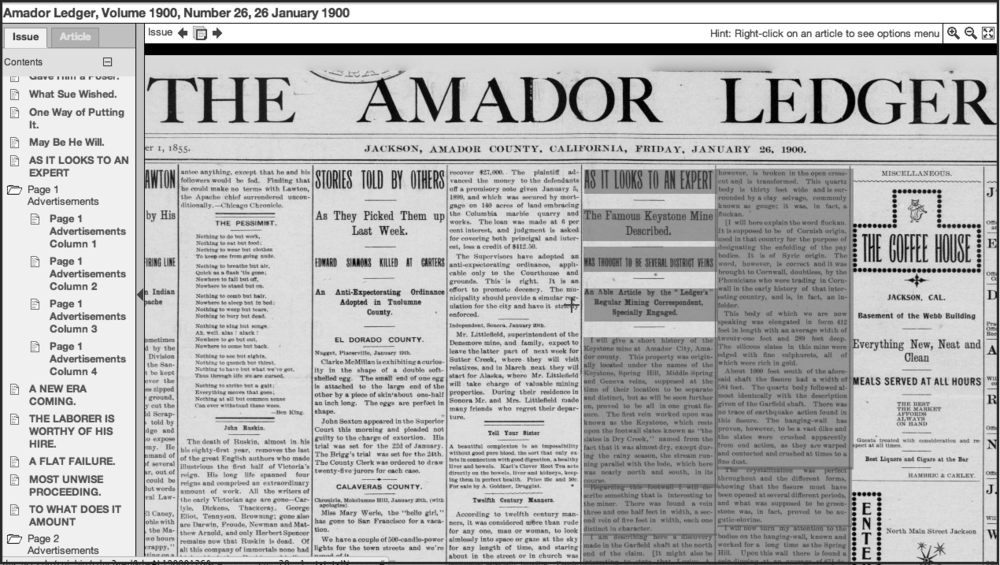
\includegraphics[width=0.48\textwidth, height=0.2\textheight]{./image/issue_greyscale.jpg}
\label{fig:T1}
}
\subfigure[The tool used by patrons to annotate articles.]
{
%%\includegraphics[width=0.8\columnwidth]{20070813-C1-7d-roc.pdf}
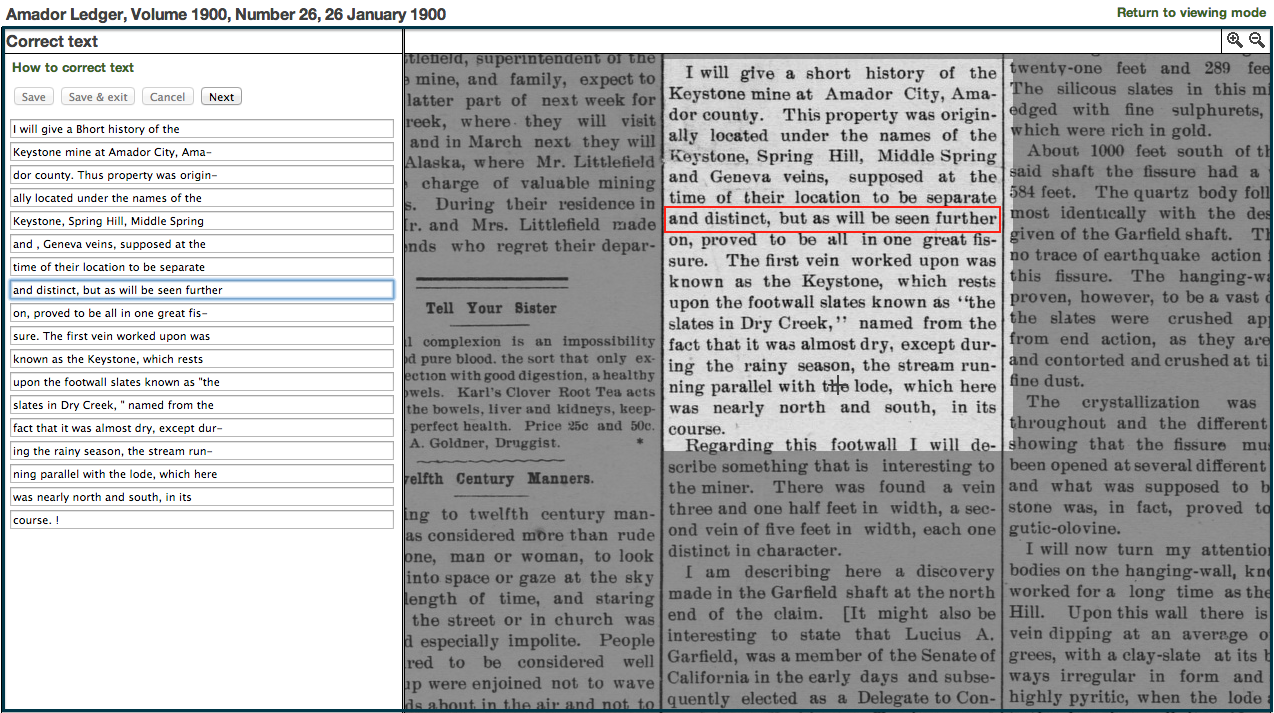
\includegraphics[width=0.48\textwidth,height=0.2\textheight]{./image/correction.jpg}
\label{fig:T2}
}
\caption{The Amador Ledger, Jan. 26, 1900.}
\label{News_01}
\end{center}
\end{figure*}

\item \textbf{Preprocessor: } The preprocessor has three main components:
\begin{itemize}
\item \textbf{Tokenizer: } The old text and the corresponding new text from the log file is tokenized by white-spaces. There are 44,022 tokens of which 20,137 are corrected by the annotators.

\item \textbf{Feature Constructor: } Features are crafted by computing the Levenshtein edit distance between the old word and its correction. The Levenshtein edit distance \cite{Wagner_74} is defined as the minimum number of single edit operations (insertions, deletions and substitutions) required to convert one string into another. Six binary features are generated as follows: 
%<<<<<<< HEAD
%
%
%\begin{enumerate}
%\item \textit{Same Length} : 1, if both the old word and new word have same length and $0$ otherwise. For example, the feature is 1 for the tokens ``Spll," and ``Union" as  both the tokens have same number of characters.
%\item \textit{Edit Distance Zero}:  1, if both the words are exactly same and $0$ otherwise. For example, the feature is 1 for tokens ``Under" and ``Under". 
%\item \textit{Edit Distance Above One}: 1, if more than one edit operation is required to convert old word to new word and $0$ otherwise. For ``Spll," and ``Union", value is 1 as more than one edit operation is required to convert from old to new token.
%\item \textit{Edit Distance Below Three}: 1, if less than three edit operations are required to convert old word to new word and $0$ otherwise. For ``Stales" and ``Stables", value is 1 as less than three edit operations are required to convert from old to new token. 
%\item \textit{Edit Distance is 1 and Case Change}: 1, if the two words have edit distance is exactly 1 and the first character of one string change from upper case to lower case or vice versa. For ``Stales" and ``Stables", the value is 0 as there are two conditions to be met. One, when both the tokens have edit distance exactly 1 and second, when there is a upper to lower or lower to upper case change in the first character. Here, the edit distance is exactly 1 but there is no case change.
%\item \textit{Punctuation Difference}: 1, if both the old text and new text differ in any of the following punctuation marks (!"\#\$\%\&'*+,-./:;\textless=\textgreater?@[$\backslash$]\^\_`\{\textbar\}\textasciitilde)
%. For ``Spll," and ``Union", the value is 1 as the old and new text differ in one of the following punctuation marks
%\end{enumerate}
%
%=======
%\begin{enumerate}
(a) \textbf{Same Length} : 1, if both the old word and new word have same length and $0$ otherwise. 
%For example, the feature is 1 for the tokens ``Spll," and ``Union" as  both the tokens have same number of characters.
(b) \textbf{Edit Distance Zero}:  1, if both the words are exactly same and $0$ otherwise. 
%For example, the feature is 1 for tokens ``Under" and ``Under". 
(c) \textbf{Edit Distance Above One}: 1, if more than one edit operation is required to convert old word to new word and $0$ otherwise. For ``Spll," and ``Union", value is 1 as more than one edit operation is required to convert from old to new token.
(d) \textbf{Edit Distance Below Three}: 1, if less than three edit operations are required to convert old word to new word and $0$ otherwise. 
%For ``Stales" and ``Stables", value is 1 as less than three edit operations are required to convert from old to new token. 
(e) \textbf{Edit Distance is 1 and Case Change}: 1, if the two words have edit distance is exactly 1 and the first character of one string change from upper case to lower case or vice versa. For example, for ``Stales" and ``Stables", the value is 0 as there is no case change.
(f) \textbf{Punctuation Difference}: 1, if both the old text and new text differ in any of the following punctuation marks (!"\#\$\%\&'*+,-./:;\textless=\textgreater?@[$\backslash$]\^\_`\{\textbar\}\textasciitilde).
% For ``Spll," and ``Union", the value is 1 as the old and new text differ in one of the following punctuation marks
%\end{enumerate}

%\begin{figure*}[t]
%\centering
%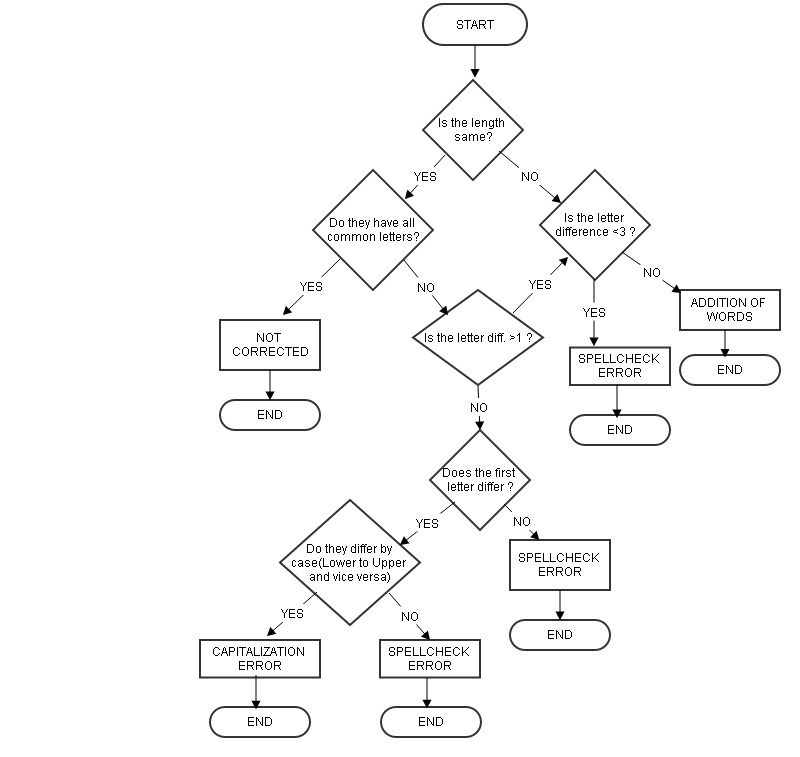
\includegraphics[width=0.9\textwidth]{./image/flowchartnew.jpg}
%%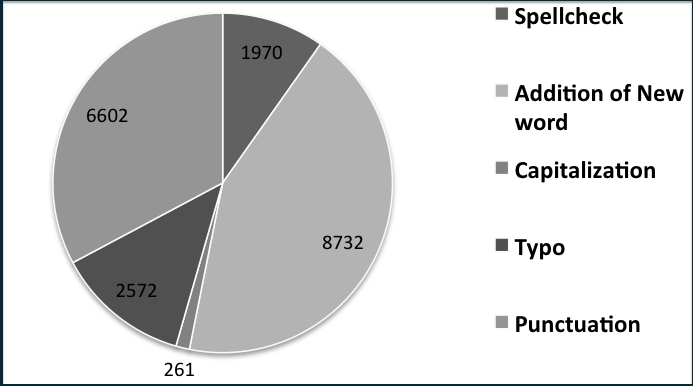
\includegraphics[width=6cm,height=4cm]{./image/error.jpg}
%\caption{Flowchart demonstrating how the labels are generated.}
%\label{fig:flowchart}
%\end{figure*}

%<<<<<<< HEAD
%\item \textbf{Label Constructor: }The errors rectified by the users are categorized as Spellcheck Error, Addition of a new word, Capitalization Error, Typo and Punctuation error. The logic used in generation of the features can be summarized by the flowchart depicted in Figure~\ref{fig:flowchart}. Specifically,
%\begin{enumerate}
%\item \textit{Class 1-Spellcheck error: }When the edit distance is between 1 and 3. For example, ``mounten" and ``mountain".
%\item \textit{Class 2-Addition of a new word: }When the edit distance is more than 3. For example, ``at" and ``attend".
%\item \textit{Class 3-Capitalization error: } When the edit distance of two strings is exactly 1 and first letter of both the strings changes from upper to lower case or vice versa. For example, ``largest" and ``Largest".
%\item \textit{Class 4-Typo: } When the edit distance is exactly one and case change is 0. For example, ``teh" and ``the"
%\item \textit{Class 5-Punctuation error: }When the two strings differ by special characters contained in the set (!"\#\$\%\&'()*+,-./:;\textless=\textgreater?@[$\backslash$]\^\_`\{\textbar\}\textasciitilde). For example, ``residents" and residents
%\item \textit{Class 6-No correction: }When the old and new text are same. For example, plant and plant
%\end{enumerate}
%
%The distribution of the these classes in the dataset is shown in Table~\ref{table: classes}.
%=======
\item \textbf{Label Constructor: }The errors rectified by the users are categorized as Spellcheck Error, Addition of a new word, Capitalization Error, Typo and Punctuation error. 
%The logic used in generation of the features can be summarized by the flowchart depicted in Figure~\ref{fig:flowchart}.
Specifically,
%\begin{enumerate}
(a)\textbf{Spellcheck Error: }When the edit distance is between 1 and 3. For example, ``mounten" and ``mountain".
(b)\textbf{Addition of a new word: }When the edit distance is more than 3. For example, ``at" and ``attend".
(c)\textbf{Capitalization error: } When the edit distance of two strings is exactly 1 and first letter of both the strings changes from upper to lower case or vice versa. For example, ``largest" and ``Largest".
(d)\textbf{Typographical Error: } When the edit distance is exactly one and case change is 0. For example, ``teh" and ``the"
(e)\textbf{Punctuation Error: }When the two strings differ by special characters contained in the set (!"\#\$\%\&'()*+,-./:;\textless=\textgreater?@[$\backslash$]\^\_`\{\textbar\}\textasciitilde). 
%For example, ``residents" and residents
(f)\textbf{No Correction: }When the old and new text are same. %For example, plant and plant
%\end{enumerate}

The distribution of the these classes in the dataset is shown in Table~\ref{table: classes}. It must be noted that by design tokens are always assigned to one class, although in principle it may be possible to assign them to multiple classes\footnote{For e.g. a correction of ``t$\$$e" to ``the" could be either a Typo or a Punctuation Error correction.}.

\begin{table}[htdp]
\begin{center}
\begin{tabular}{| c | c |}
\hline
 Class  & No. of Instances \\
\hline
 Spellcheck & 1970 \\
%\hline 
 Addition of new word & 8732 \\
%\hline
 Capitalization & 261 \\
%\hline
Typo & 2572 \\
%\hline
Punctuation & 6602 \\
%\hline
No correction & 23885 \\
\hline
Total & 44022 \\
\hline
\end{tabular}
\end{center}
\caption{Class Distribution}
\label{table: classes}
\end{table}

\end{itemize}
%\begin{figure}[h]
%\centering
%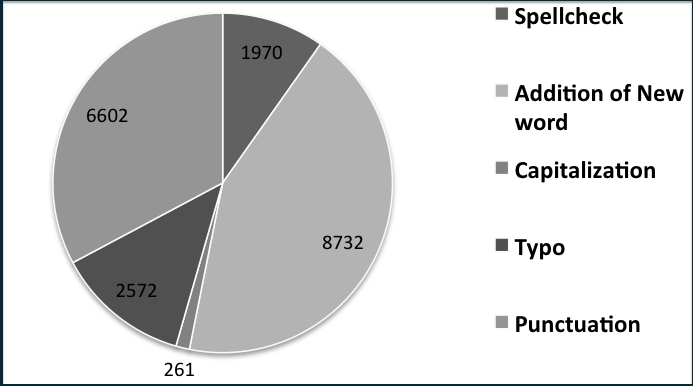
\includegraphics[width=0.48\textwidth]{./image/error.jpg}
%%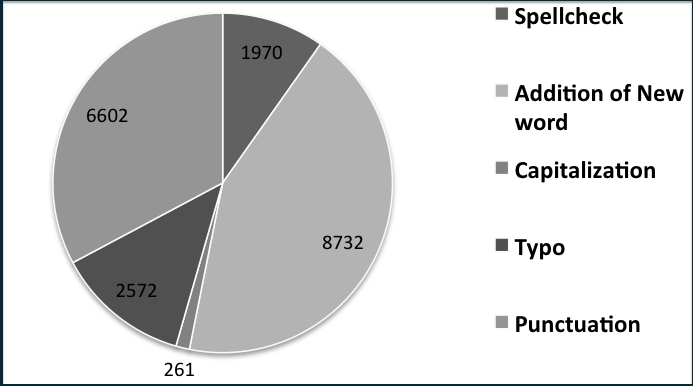
\includegraphics[width=6cm,height=4cm]{./image/error.jpg}
%\caption{Error Classification}
%\label{fig:stats}
%\end{figure}


%The error classes were restricted to 6 classes including Spellcheck Error, Addition of a new word, Capitalization Error, Typo, Punctuation Error and No correction



%The dataset was parsed to a format used by the Joachim's multi class SVM algorithm which is represented as\\
%\textless target\textgreater\space\textless feature\textgreater:\textless value\textgreater ......\textless feature\textgreater:\textless value\textgreater\\
%The number of rows in the dataset is 44,022. 
%The class distribution in the dataset is shown in table ~\ref{table: classes}

%


%<<<<<<< HEAD
%\item \textbf{Model Construction: } The crowdsourced text correction model is built using a Multiclass Support Vector Machine algorithm \cite{algo}. For a training set $(x_1,y_1) ... (x_n,y_n)$ with labels $y_i \in \{1, \cdots, k\}$, the multi class problem is posed as a constrained optimization problem with a quadratic objective function which can be stated as: \\
%\begin{equation}
%\text{min } \frac{1}{2} \sum_{i = 1}^{k} \parallel w_{i}\parallel^2 + \frac{C}{n} \sum_{i = 1}^{n}\xi_{i} 
%\end{equation}
%\begin{equation*}
%s.t. \forall y \leq k : [x_{1} \cdot w_{yi}] \geq [x_{1} \cdot w_{y}] + 100*\Delta(y_{1},y)-\xi_{1}
%\end{equation*}
% . . . . . . . . . . .
%\begin{equation*}
%s.t. \forall y \leq k : [x_{n} \cdot w_{yn}] \geq [x_{n} \cdot w_{y}] + 100*\Delta(y_{n},y)-\xi_{n} 
%\end{equation*}
%Here C is the regularization parameter that trades off margin error and training error. $\Delta(y_{1},y)$ is the loss function that returns 0 if $y_{n}$ equals y, and 1 otherwise. $\xi_{i}$ are the non negative slack variables which measure the degree of misclassification of the data $x_{i}$. \\
%\cite{algo} has two modules, \textit{svm\_multiclass\_learn} and \textit{svm\_multiclass\_classify}. The learning module learns the model given the parameters and the training data whereas the classification module applies the learned model to the test data to find the error. When the data is not linearly separable, the original finite dimensional space is mapped to a much higher dimensional space in order to make the separation easier in that space. The mappings used by SVM schemes are designed to ensure that the dot products may be computed easily in terms of the variables in the original space, by defining them in terms of a Kernel function selected to suit the problem. The types of kernel function used can be described as follows:\\
%a) Linear Kernel (default) : It is the basic kernel function given by the inner product \textless x,y\textgreater plus an optional constant c. K(x,y) = $x^{T}$y + c \\
%b) Polynomial Kernel : It is a non-stationary kernel which is well suited for problems where the training data is normalized. \\
%K(x,y) = $(\alpha x^{T}y + c)^{d}$ \\
%c) Radial Basis Kernel : The (Gaussian) radial basis function kernel on two samples x and y represented as feature vectors in some input space is defined as \\
%K(x,y) = exp($-\lvert \lvert x-y\rvert\rvert^{2}$/2$\sigma^{2}$)
%=======
\item \textbf{Model Construction: } The model for classifying crowdsourced text correction is built using a Multiclass Support Vector Machine algorithm \cite{Tsochantaridis_2004}. Each training point belongs to one of $k$ different classes. The goal is to construct a function, which given a new data point, will correctly predict the class to which it belongs.
Different methods have been proposed in literature for solving the SVM multi-class classification problem. Some popular techniques include: a) \textit{One-Versus-All (OVA) classification} Build $k$ different binary classifiers; for the $i^{th}$ classifier, let the positive examples be all points in class $i$ and negative examples not in class $i$. Let $f(x) = \text{arg } max_i f_i(x) $.  b) \textit{one-versus-one} uses the majority voting strategy where each classifier assigns the new instance one of two classes. The class with the majority votes is assigned to the instance.
%%It generates k(k-2)/2 models for a k class problem. This approach is not practical for large-scale classification because of the memory required for storing k(k-1)/2 models.
%c) \textit{Directed Acyclic Graph SVM} in its training phase, it is the same as the one-vs-one method. However, in the testing phase, it uses a rooted binary directed acyclic graph which has k(k-1)/2 internal nodes and k leaves. 
%d) \textit{Error Correcting Output Codes} \cite{multiclassSVM_ecoc} This technique tries to combine binary classifiers by using decorrelations and correct errors.
Crammer and Singer \cite{crammer} pose the multi-class classification problem as a single optimization problem, rather than decomposing it into multiple binary classification problems. A comparison of the above approaches can be found here \cite{comparison}.

For a training set $(x_1,y_1) ... (x_n,y_n)$ with labels $y_i \in \{1, \cdots, k\}$, the multi class problem can be posed as a constrained optimization problem with a quadratic objective function:
$\text{min } \frac{1}{2} \sum_{i = 1}^{k} \parallel w_{i}\parallel^2 + \frac{C}{n} \sum_{i = 1}^{n}\xi_{i} $

s.t. $\forall y \leq k : [x_{1} \cdot w_{yi}] \geq [x_{1} \cdot w_{y}] + 100*\Delta(y_{1},y)-\xi_{1}$
$\cdots$
s.t. $\forall y \leq k : [x_{n} \cdot w_{yn}] \geq [x_{n} \cdot w_{y}] + 100*\Delta(y_{n},y)-\xi_{n}$

Here $C$ is the regularization parameter, $\Delta(y_{j},y), 1 \le j \le n$ is the loss function that returns 0 if $y_{j}$ equals y, and 1 otherwise and $\xi_{i}, 1 \le i \le n$ are the non negative slack variables which measure the degree of misclassification of the instance $x_{i}$. 
%\cite{algo} has to two modules, \textit{svm\_multiclass\_learn} and \textit{svm\_multiclass\_classify}. The learning module learns the model given the parameters and the training data whereas the classification module applies the learned model to the test data to find the error. 
It must be noted that when the data is not linearly separable, the following kernel functions are used for classification:
%the original finite dimensional space is mapped to a much higher dimensional space in order to make the separation easier in that space. The mappings used by SVM schemes are designed to ensure that the dot products may be computed easily in terms of the variables in the original space, by defining them in terms of a Kernel function selected to suit the problem. The types of kernel function used can be described as follows:\\
a) Linear Kernel: $K(x,y) = x^{T}y + c $
b) Polynomial Kernel : $K(x,y) = (\alpha x^{T}y + c)^{d}$
c) Radial Basis Kernel : $K(x,y) = exp(-\lvert \lvert x-y\rvert\rvert^{2}/2\sigma^{2}$)

%
\item \textbf{Information Retrieval Techniques: } The tokens identified by the model as ``spell check",``addition of a new word", and ``Typo" play an important role in trying to enhance search and retrieval on the archive. This is presented here for the completeness of the architecture, but described in detail in Section~\ref{ir}.




\end{enumerate}

\section{Empirical Evaluation}
\label{sec:evaluation}

Experiments are performed by randomly selecting $70\%$ of the data\footnote{Approximately 30,815 instances}  as the train set. For each experiment, the regularization parameter $C$ and the type of kernel $t$ are varied as $0.001,0.01,0.1,1,10,100$ and Linear, Polynomial and Radial Basis Function kernel respectively. The experiments are performed on two machines, one of which is a linux server and the other a dual core Mac machine with Intel Core i7 processor, 8GB RAM, 2.9 GHz of processor speed. Each experiment is repeated $5$ times and the average loss on the test set and CPU runtime are reported. Table ~\ref{table: error} presents the average loss on test set for different values of $C$ and $t$; $AE_{L}$, $AE_{P}$, $AE_{R}$ represents the average loss on the linear, polynomial and RBF kernels respectively. Table ~\ref{table: runtime} shows the average runtime (cpu sec) required to learn a model for various values of $C$ and for different kernels. Here, $AT_{L}$, $AT_{P}$, $AT_{R}$ refers to the average run time of linear, polynomial and rbf kernels respectively. The loss is least when the $C = 100$ for the polynomial kernel. However, the time taken to train the model is considerably higher at 106753s. It must also be noted that one can learn less accurate models with linear or RBF kernels faster. Thus, it may be useful to consider a trade-off between accuracy of learnt models versus time taken for classification in large scale deployments.
 
The code used to build the prototype system along with data generated are available from \texttt{https://github.com/megha89/}. It must be noted that the $SVM^{multiclass}$V2.2 package \cite{algo} was used for the implementation of Multi-class SVMs. 
For linear kernels, $SVM^{multiclass}$V2.20 is very fast and runtime scales linearly with the number of training examples. Training of non-linear kernels is very slow using the algorithm described in Section~\ref{arch}.

%\subsection{Results}

\begin{table}[htdp]
\begin{center}
\begin{tabular}{| c | c | c | c |}
\hline
C & $AE_{L}$ & $AE_{P}$ & $AE_{R}$ \\
\hline
.001 & 32.06 $\pm$0.149  & 32.06$\pm$0.149 & 11.96$\pm$0.101 \\
.01 & 32.06$\pm$0.149 & 32.06$\pm$0.149 & 12.04$\pm$0.199 \\
.1 & 32.06$\pm$0.149 & 29.10$\pm$0.133  & 12.04$\pm$0.199  \\
1 &29.10$\pm$0.133  & 28.99$\pm$0.264  & 6.36$\pm$0.142  \\
10 & 29.20$\pm$0.133 & 8.338$\pm$0.107 & 6.36$\pm$0.142 \\
100 & 29.20$\pm$0.133 & 0.58$\pm.034$ & 6.35$\pm0.16$  \\
\hline
\end{tabular}
\end{center}
\caption{Experiment Results : Average loss error (test set)}
\label{table: error}
\end{table}


\begin{table}[htdp]
\begin{center}
\begin{tabular}{| l | c | c | l |}
\hline
C & $ AT_{L} $ & $AT_{P}$ & $AT_{R}$ \\
\hline
.001 & 0.218 & 5192 & 4596 \\
.01 & 0.202 & 5166 & 4460 \\
.1 & 0.208 & 72225 & 4377 \\
1 & 0.678 & 81251 & 16468 \\
10 & 0.672 & 260316 & 55308 \\
100 & 0.998 & 106753  & 48734  \\
\hline
\end{tabular}
\end{center}
\caption{Experiment Results : Training time (cpu sec)}
\label{table: runtime}
\end{table}

%\subsection{Discussion}

%\subsection{Known Defects}
%The \cite{algo} algorithm converges quickly for linear type kernel but the its performance on test set is poor. For non linear kernels, this algorithm does not scale well for large scale datasets but gives better performance than linear kernels.

\section{Information Retrieval Techniques}
\label{ir}
The following details are relevant: 

\noindent \textbf{Query Set:} To measure the retrieval effectiveness of the corrected text versus the garbled OCR, a list of keywords for search was prepared by randomly sampling from the corrected words.

\noindent \textbf{Software:} PyLucene 3.6.2, a Python extension for accessing Java Apache Lucene was used as an IR software library for enabling full text indexing and search capabilites. Inverted indices are built for both the original and corrected corpus. Keywords from the query set are tested on both corpora and documents containing words in the query set are retrieved. The documents are ranked according to the frequency of the keyword present -- higher the frequency, higher the rank.
 
\noindent \textbf{Evaluation:} The metric used to compare the retrieved documents is Spearman's rank correlation coefficient($\rho$). Let $y_{i}$ be the rank ordering of the documents retrieved from the corrected corpus and $x_{i}$ the rank ordering for the garbled text. Let $d_{i}$ = $x_{i}$ - $y_{i}$. Then Spearman's rank correlation $\rho$ is given by: $\rho = 1 - \frac {6\sum d_i^2 }{n(n^2-1)}$.

\noindent \textbf{Example: } Query word ``Jackson", the evaluation of $\rho$ is shown in Table~\ref{ex}. Here, ${\sum d_i^2}$ = 11 and $\rho$ = 0.45.
\begin{table}[h]
\centering
\begin{tabular}{ l | c | c | c | r | r }
 $Y_{i}$ & $X_{i}$ & $y_{i}$ & $x_{i}$ & $d_{i}$ & $d_{i}^2$ \\
\hline
  12-01-1900 & 21-10-1910 & 1 & 10(4) & -3 & 9 \\
  09-12-1910 & 09-12-1910 & 2 & 2(1) & 0 & 0 \\
  08-06-1900 & 23-09-1910 & 3 & 7(2) & 1 & 1 \\
  01-04-1904 & 02-12-1910 & 4 & 8(3) & 1 & 1 \\
  25-05-1900 & 23-12-1910 & 5 & 11(5) & 0 & 0 \\
\end{tabular}
\label{ex}
\end{table}

\noindent \textbf{Deployment: }The full-scale deployment of this prototype system is being considered on old historic newspaper archives at California Digital Newspaper Collection and the New York Public Library among others, where  user text corrections are used extensively for cleaning garbled OCR. 

\section{Related Work}
\label{sec:related}
\noindent \textbf{Optical Character Recognition (OCR)} is a commonly used method of digitizing printed texts so that it can be searched and displayed online, stored compactly and used in text mining applications. The text generated from OCR devices is often garbled due to variations in quality of the input paper, size and style of the font and column layout, its condition at the time of microfilming, choice of scanner, and the quality of the OCR software. Several techniques for post processing garbled OCR have been designed \cite{Fujisawa_08}, \cite{Esakov_94}, \cite{Lecun_90}. These include:

\noindent \textbf{Dictionary based schemes: }These algorithms use a dictionary to spellcheck misspelled OCR recognized words. They correct non-word errors - words that are recognized by the OCR device but do not correspond to any entry in the lexicon. Niwa et al. \cite{postprocessing} proposed an OCR post error correction method based on pattern learning where a list of suitable candidates is generated from the lexicon and the best candidate is selected as a correction. Yannakoudakis and Fawthrop \cite{Yannakoudakis_83} conducted a study to create a set of rules based on common misspelling pattern and used them to correct errors. Cherkassky and Vassilas \cite{Cherkassky_89} use back propagation algorithms for correction. 
%\cite{statistical} proposed using Hidden Markov Models (HMMs) to integrate syntactic information into the post-processing error correction. 
%The suggested model achieved a higher rate of error correction due to its statistical nature in selecting the most probable candidate for a particular misspelled word.

\noindent \textbf{Context based schemes: }These algorithms perform error detection and correction based on the grammatical error and semantic context. They are able to correct real-word errors -- words that are recognized by the OCR system and correspond to an entry in the lexicon. Tong and Evans \cite{Tong96astatistical} describe an automatic, context-sensitive, word-error correction system based on Statistical Language Modeling (SLM). The system exploits information from letter n-grams, character confusion probabilities and word bi-gram probabilities. Golding et al. \cite{contextbased} applies a part-of-speech (POS) tagger enhanced by word trigram model and a statistical Bayesian classifier to correct real-word errors in OCR text. Reynaert \cite{Reynaert2008a} presents a system for reducing the level of OCR-induced typographical variation in large text collections called Text-Induced Corpus Clean-up (TICCL). The system focuses on high-frequency words to be cleaned and gathers all typographical variants for any particular focus word that lie within the predefined Levenshtein distance. Bassil et al. \cite{Bassil_12a,Bassil_12b} propose a post-processing context-based error correction algorithm for detecting and correcting OCR non-word and real-word errors. The proposed algorithm is based on Google's online spelling suggestion. Abdulkader et al. \cite{lowcost}  present a method for digitizing textual data by using neural network classifiers to estimate OCR errors, clustering similar errors, designing a user interface and using active learning to tune the error estimation from user labeled data. 
Velagapudi \cite{velagapudi} uses a combination of classifiers -- kNN classifier,  multilayer perceptrons and SVM to discuss the effects of error correction on the classification accuracy of each method. 

Very little work has been done on automatic \emph{classification} of OCR error corrections\footnote{Most prior work has dealt with evaluation of candidate corrections for OCR errors.} to get a clear understanding of the \emph{nature} of errors encountered -- Esakov et al. \cite{Esakov_94a} suggest classification of output from the OCR engine as simple substitutions ($e \rightarrow c$), improper segmentation or multiple substitutions $(T \rightarrow 'l, m \rightarrow rn, he \rightarrow b)$, deletions and insertions (involving space) and unrecognized characters $(u \rightarrow \sim)$. They use a new variant of the dynamic programming algorithm for classification. In \cite{hybred}, OCR documents are classified into fixed number of categories based on their content. The accuracy of their approach was best when evaluated using SVM among other algorithms. Daoason \cite{Jon_12} posits that OCR errors are not random -- for example, it is extremely unlikely that the letter $o$ will be misrecognized as $x$ since they are very dissimilar. He classifies OCR errors as character errors (characters in the input document that are replaced with other characters), word errors (word in the input document is not correct or not present in the OCR generated text), or zoning errors (OCR software is unable to decipher zones correctly). Our work primarily focusses on \emph{manual} error correction classification where the task of correcting OCR errors is outsourced to a crowd of workers. 
%By engaging a large crowd of people for ideas, skills or participation the quality of work done is superior and relatively inexpensive.

%It is estimated that the total count of published books in the world is around 130 million \cite{bookscount}. Many of these books published are only available in printed format due to reasons like copyright and licensing issues. This limits the search of these articles, their availability and accessibility on the web. As of 2013, more than 30 million books have been digitised by Google Books Library Project \cite{gblp}. It uses reCAPTCHA to digitise books one word at a time by sending words that can not be read by the computer to the web in the form of CAPTCHAs for humans to decipher \cite{recaptcha}. 

%The OCR enables searching of full text data but it is not 100\% accurate. Its accuracy largely depends on paper quality of the original issue, font style, column layouts, its condition at the time of microfilming, choice of scanner \cite{issue}, and the quality of the OCR software. The OCR errors are widely classified as non-word errors and real-word errors. A non-word error takes place when the erroneous word is not a dictionary word whereas in real-word error the erroneous word is correctly spelt and therefore can be found in the dictionary but incorrectly used in context.
%The error generated by OCR can be classified in several categories. One such classification similar to ours is done by \cite{post-correction}. It gives an exhaustive error classification that helps in classifying real words , that is words that are not contained in any of the dictionary, e.g. names, out-dated or historic spelling variations. Segmentation errors, Hyphenation error, Misrecognition of characters, Punctuation errors, Case sensitivity, Changed word meaning are the classes required for better classification of OCR errors.

%The OCR errors are usually dependent on some major factors like the page quality, text layout, font styles. In \mydoubleq{Issues in automatic error correction}, the experimental analysis has shown that there is another important factor that impacts the performance of the OCR errors which is the choice of scanners used to scan the printed text. The type of scanner used not only affect the quantity of errors but quality as well. Their algorithm for classifying OCR errors is based minimising the cost of basic operations used to transform one string to another, also known as edit distance using dynamic programming approach.\\
%\mydoubleq{Unsupervised Post Correction} paper talks about the post processing of OCR text to minimise the errors. It uses a combination of Anagram Hashing techniques, bigram approach on word level to consider the context and a  similarity key technique called OCR-key.  Anagram Hashing technique uses a hashing function that assigns same number to all those words that have same characters. OCR key observes the shape of characters to know the nature of OCR system and its generated errors.
\noindent \textbf{Crowdsourced OCR correction }Recruiting users and paying them small sums of money to tag and annotate text and images in large digital archives has become common practice (e.g. Amazon's Mechanical Turk, reCAPTCHA \cite{vonAhn_08}, ESP \cite{vonAhn_04}) and Games with a Purpose \cite{Ahn_08w}. A number of recent papers have evaluated the effectiveness of using Mechanical Turk to create annotated data for text and natural language processing applications \cite{Snow_08}. In the same vein, many workshops and conferences have been organized on the theme of machine learning in human computation, crowdsourcing and collective intelligence\footnote{See http://ir.ischool.utexas.edu/crowd/}. 

Intuitively, the easiest way to correct garbled OCR text is to hire a group of people to edit it manually. Distributed Proofreaders (DP) \cite{DP} is a web-based project designed to facilitate proofreading of paper books into e-books and was meant to assist the project Gutenberg\footnote{http://www.gutenberg.org/}. Wikipedia is yet another example of a large scale crowdsourcing project. Yamangil et al. \cite{wikiedits} proposed a learning algorithm for mining wikipedia edit history using baseline Hidden Markov Model augmented with perceptron re-ranking. The model was trained on wikipedia edits and hence incorporated human corrections. 
%\subsection{Multi-class SVM}



\section{Conclusion \& Future Work}
\label{sec:conc}
The California Digital Newspaper Collection has an archive of 400,000 pages of historical California newspapers published between 1846 to 1922. This archive which has been subjected to OCR and is currently stored in an online database making them accessible to patrons. The OCR scanning process generates lot of garbled text which needs to be corrected to make the online newspaper repository more accessible to general public. 

In this paper, we present a system for Classification of Crowdsourced Text Correction which is capable of modeling user corrections using state-of-the-art machine learning techniques and retrieve categories which are likely to enhance search on the archive such as addition of words, elimination of typographical errors or addition of content. Information retrieval metrics are used to quantify the effectiveness of the user text correction. The prototype system is being considered for deployment on historic newspaper archives at the California Digital Newspaper Collection and the New York Public Library.

% use section* for acknowledgement
\section*{Acknowledgment}
This work is supported by funding from the National Endowment for Humanities, Grant No: NEH HD-51153-10. The authors would like to thank Stefan Boddie, DL Consulting, Ltd., New Zealand for sharing experiences with the Veridian software and Luis. C. Baquera, University of California, Riverside for providing data generated from the log files at CDNC.\\


\bibliographystyle{aaai}
\bibliography{flairsPaper}
\end{document}
